\documentclass[tikz, border=10pt]{standalone}
\usepackage{tikz}
\usepackage{amsmath}
\usetikzlibrary{calc, arrows.meta}

\begin{document}
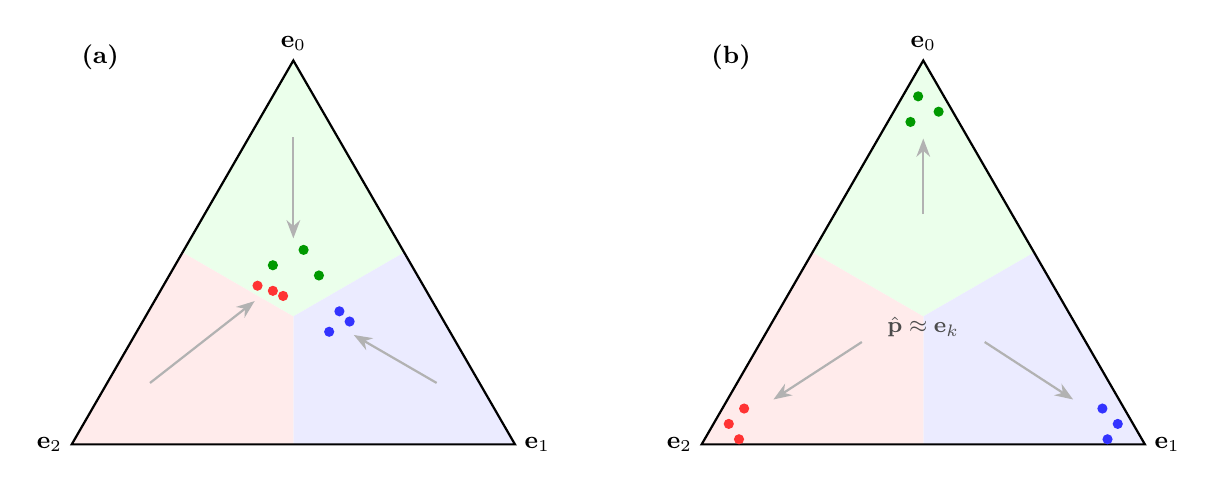
\begin{tikzpicture}[font=\sffamily]

    % ===== LEFT PANEL: Oversmoothing =====
    \begin{scope}[scale=0.65]
        % Vertices
        \coordinate (T) at (0, 5);
        \coordinate (R) at (4.33, -2.5);
        \coordinate (L) at (-4.33, -2.5);

        % Centroid and edge midpoints
        \coordinate (G) at (0, 0);
        \coordinate (MidTR) at (2.165, 1.25);
        \coordinate (MidTL) at (-2.165, 1.25);
        \coordinate (MidRL) at (0, -2.5);

        % Light region fills (same as 0/1 loss partition)
        \fill[green!8] (T) -- (MidTR) -- (G) -- (MidTL) -- cycle;
        \fill[blue!8] (R) -- (MidRL) -- (G) -- (MidTR) -- cycle;
        \fill[red!8] (L) -- (MidTL) -- (G) -- (MidRL) -- cycle;

        % Triangle frame
        \draw[thick] (T) -- (R) -- (L) -- cycle;

        % Contraction arrows (showing direction of distortion toward centroid)
        \draw[->, >=Stealth, gray!60, thick, shorten >=6pt] (0, 3.5) -- (0, 1.2);
        \draw[->, >=Stealth, gray!60, thick, shorten >=6pt] (2.8, -1.3) -- (0.9, -0.2);
        \draw[->, >=Stealth, gray!60, thick, shorten >=6pt] (-2.8, -1.3) -- (-0.5, 0.5);

        % Estimated points colored by TRUE class, all clustered near centroid
        % Class 0 (green) — estimates still in R_0
        \node[circle, fill=green!60!black, inner sep=1.3pt] at (0.2, 1.3) {};
        \node[circle, fill=green!60!black, inner sep=1.3pt] at (-0.4, 1.0) {};
        \node[circle, fill=green!60!black, inner sep=1.3pt] at (0.5, 0.8) {};

        % Class 1 (blue) — estimates still in R_1
        \node[circle, fill=blue!80, inner sep=1.3pt] at (0.9, 0.1) {};
        \node[circle, fill=blue!80, inner sep=1.3pt] at (0.7, -0.3) {};
        \node[circle, fill=blue!80, inner sep=1.3pt] at (1.1, -0.1) {};

        % Class 2 (red) — estimates in R_0, NOT in R_2 (misclassified)
        \node[circle, fill=red!80, inner sep=1.3pt] at (-0.4, 0.5) {};
        \node[circle, fill=red!80, inner sep=1.3pt] at (-0.2, 0.4) {};
        \node[circle, fill=red!80, inner sep=1.3pt] at (-0.7, 0.6) {};

        % Vertex labels
        \node[above, font=\small] at (T) {$\mathbf{e}_0$};
        \node[right, font=\small] at (R) {$\mathbf{e}_1$};
        \node[left, font=\small] at (L) {$\mathbf{e}_2$};

        % Panel label
        \node[font=\small\bfseries, anchor=north west] at (-4.33, 5.5) {(a)};
    \end{scope}

    % ===== RIGHT PANEL: Undersmoothing =====
    \begin{scope}[xshift=8cm, scale=0.65]
        % Vertices
        \coordinate (T) at (0, 5);
        \coordinate (R) at (4.33, -2.5);
        \coordinate (L) at (-4.33, -2.5);

        % Centroid and edge midpoints
        \coordinate (G) at (0, 0);
        \coordinate (MidTR) at (2.165, 1.25);
        \coordinate (MidTL) at (-2.165, 1.25);
        \coordinate (MidRL) at (0, -2.5);

        % Light region fills
        \fill[green!8] (T) -- (MidTR) -- (G) -- (MidTL) -- cycle;
        \fill[blue!8] (R) -- (MidRL) -- (G) -- (MidTR) -- cycle;
        \fill[red!8] (L) -- (MidTL) -- (G) -- (MidRL) -- cycle;

        % Triangle frame
        \draw[thick] (T) -- (R) -- (L) -- cycle;

        % Expansion arrows (showing direction of distortion toward vertices)
        \draw[->, >=Stealth, gray!60, thick, shorten >=6pt] (0, 2.0) -- (0, 3.8);
        \draw[->, >=Stealth, gray!60, thick, shorten >=6pt] (1.2, -0.5) -- (3.2, -1.8);
        \draw[->, >=Stealth, gray!60, thick, shorten >=6pt] (-1.2, -0.5) -- (-3.2, -1.8);

        % Data points clustered near vertices (overconfident)
        % Class 0 near Top
        \node[circle, fill=green!60!black, inner sep=1.3pt] at (-0.1, 4.3) {};
        \node[circle, fill=green!60!black, inner sep=1.3pt] at (0.3, 4.0) {};
        \node[circle, fill=green!60!black, inner sep=1.3pt] at (-0.25, 3.8) {};

        % Class 1 near Right
        \node[circle, fill=blue!80, inner sep=1.3pt] at (3.8, -2.1) {};
        \node[circle, fill=blue!80, inner sep=1.3pt] at (3.5, -1.8) {};
        \node[circle, fill=blue!80, inner sep=1.3pt] at (3.6, -2.4) {};

        % Class 2 near Left
        \node[circle, fill=red!80, inner sep=1.3pt] at (-3.8, -2.1) {};
        \node[circle, fill=red!80, inner sep=1.3pt] at (-3.5, -1.8) {};
        \node[circle, fill=red!80, inner sep=1.3pt] at (-3.6, -2.4) {};

        % Annotation
        \node[black!70, font=\footnotesize, align=center] at (0, -0.2)
            {$\hat{\mathbf{p}} \approx \mathbf{e}_k$};

        % Vertex labels
        \node[above, font=\small] at (T) {$\mathbf{e}_0$};
        \node[right, font=\small] at (R) {$\mathbf{e}_1$};
        \node[left, font=\small] at (L) {$\mathbf{e}_2$};

        % Panel label
        \node[font=\small\bfseries, anchor=north west] at (-4.33, 5.5) {(b)};
    \end{scope}

\end{tikzpicture}
\end{document}
